% file to contain information on examples
%==============================================================================
\chapter{Examples Explained - WIP}
Examples are located in the \verb|0-examples| folder and are designed to be run in batch mode.
This means that each example copies any required system, model, or modulation file to the main PST directory before running.
Typically, each example folder contains a \verb|.m| file that starts with \verb|run| that can be used to run the example.
As example cases are located on a github repository, relative file paths are used so that examples can be run without much difficulty from various different machines.
While most examples can be run in multiple versions of PST, some functionality can only be found in specific versions.

\noindent The general structure of created examples tend to reflect the following:
\begin{enumerate}
\itemsep 0em
\item Clear all variables, close all figures, and clear the command window
\item Define which version of PST to use
\item Create a relative path to the root directory of chosen PST version
\item Copy any system, model, or modulation file to the PST root directory
\item Run \verb|s_simu|
\item Save output data
\item Restore any model, or modulation file to original state
\item Create data plots
\end{enumerate}

%=================================================================
\pagebreak
\section{Standard Faulting (hiskens)}
Standard PST simulations involve some kind of fault defined in the \verb|sw_con| array.
This example (located in the \verb|hiskens| folder) is included to showcase some simple differences between PST versions using a standard test case.
System data for this example comes from a report by Ian Hiskens \cite{hiskens2013} which summarized a study of an IEEE 10 generator, 39 bus system.
Ryan Elliott at Sandia National Labs recreated the system in a PST format and provided the data file for this project.
A one-line diagram of the system is shown in Figure \ref{fig: hiskens oneline}.

\begin{figure}[H]
	\centering
	\footnotesize
	\includegraphics[width=.85\linewidth]{figures/hiskens/hiskensOneline}
	\caption{IEEE 39 bus network.}
	\label{fig: hiskens oneline}
\end{figure}%\vspace{-1 em}

The simulated event was a 0.1 second three-phase fault with no loss of line between bus 2 and 3.
The \verb|run_datane_hiskens.m| file can be used to run the simulation.
Figure \ref{fig: hiskens results} shows the resulting fault bus voltage magnitude and system generator speeds.

\begin{figure}[H]
	\centering
	\footnotesize
	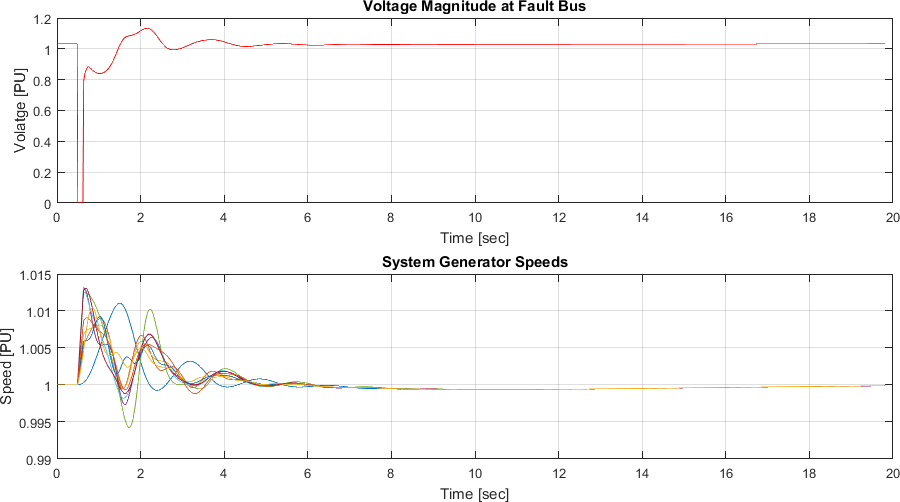
\includegraphics[width=\linewidth]{figures/hiskens/hiskensResults}
	\caption{Hiskens Example Fault Bus Voltage and Generator Speeds.}
	\label{fig: hiskens results}
\end{figure}%\vspace{-1 em}

All PST versions (when using the same models) provide the same results, but there are differences in simulation speed and data output.
Table \ref{tab: hiskens} shows that the PST 4 simulation was roughly twice as fast as PST version 2 or 3, saved less data, and left fewer variables in the MATLAB workspace post simulation.
These improvements are likely due to the restructuring of global variables and code to remove any `all zero` data from being saved.\\

% table data for hiskens fault comparison 


\begin{table}[H]
%\resizebox{\linewidth}{!}{ % Use to resize large tables
\singlespacing
	\begin{tabular}{@{} L{1.75cm} 
	R{2cm} R{2cm}  R{2cm} @{}} 	
		\toprule % @ signs to remove extra L R space
		\footnotesize % this will affect the table font (makse it 10pt)
		\raggedright % for non justified table text
						
										
										
		PST Version	&	Simulation Time [seconds]	&	Resulting Workspace Variables	&	Saved Data Size [KB]	\\ \midrule	
		2.3	&	16.56	&	206	&	7,549	\\	
		3.1	&	16.70	&	210	&	7,548	\\	
		SETO	&	8.42	&	24	&	3,965	\\	
		4	&	7.96	&	6	&	3,974	\\	\bottomrule

													
	\end{tabular}

	\caption{PST Version Comparisons of Hiskens Example.}
	\label{tab: hiskens}
%	}%end resize box
\end{table}


%=====================================================================
\section{Modulation Examples - WIP} \label{sec: modExamples}
PST provides numerous ways to input a defined modulation signal into a variety of models.
The following list of example folder names work in all versions of PST and typically create linear/non-linear comparison plots.
While the examples themselves do not reflect any particular scenario, the provided code may be useful in creating particular scenarios.

\begin{itemize}
\item \verb|lmod| - Uses the \verb|ml_sig| file to modulate real load power.
\item \verb|mexc| - Uses the \verb|mexc_sig| file to modulate the exciter reference signal.
\item \verb|mtg_sig| - Uses the \verb|mtg_sig| file to modulate the governor $P_{ref}$ reference signal.
\item \verb|pm_sig| -Uses the \verb|mpm_sig| file to modulate a machines mechanical power.
\item \verb|rlmod| - Uses the \verb|rml_sig| file to modulate a load's reactive power.
\item \verb|SVC| - Uses the \verb|msvc_sig| file to modulate an SVC's output value.
\item \verb|TCSC| - Uses the \verb|mtcsc_sig| file to modulate an TCSC's output value.
\end{itemize}

\noindent It should be noted that modulation files for PST 2 and 3 assume input to function is ($t, k$), i.e. full time vector and data index, while PST 4 only requires the data index $k$.

%=====================================================================
% all current examples
\pagebreak
All un-categorized examples from 0-examples folder are listed below - last bit of User manual work will be to `thin the herd', insert previous results, confirm working, and provide minor details about content


\section{AGC - WIP}
PST 4 only

\subsection{run\_AGC - WIP}
- 2 area kundur with optional integration methods = load step - 120 second recovery.

\subsection{run\_AGC\_mod - WIP}
  - same system as above - uses Interchange modulation signal as perturbance


\section{DC - WIP}
All versions - 

non-linear simulation seems to work

linear analysis doesn't seem to work correctly - user error?


\section{exciterBatchTests - WIP}
PST 4 only - used to compare all 4 exciter models linear/non-linear response to load step

Was useful in ensuring exciter models were cast to globals correctly

\section{extendedTerm - WIP}
Results written up in 200806-ExtendedVersionComp


\section{inductive - WIP}
meant to verify functionality of inductive generators and loads (motors)

Multiple cases run from example script: fault example and load pulse with linear/non-linear comparison.
Works in all versions.

\section{ivmmod - WIP}
example modified from Dan - includes a VTS example  -
requires some minor reworking - 

shows how angle change `moves' entire system.

VTS method used - clearly shows how variable time steps adjust to capture dynamics

\section{miniWECC - WIP}

	\subsection{AGC - WIP} 
multi area agc (VTS?)

	\subsection{genTrip - WIP} 
use to show arbitrary tripping



\section{pwrmod -WIP} \label{sec: pwrmodExamples}
\subsection{P-injection - WIP}
\subsection{I-injection - WIP}


\section{untrip - WIP}
Documentation created in\\ \verb|MT-Tech-SETO\researchDocs\TEX\one-offs\200901-refinedUntripResults2|

Variables to note in associated examples (where \verb|x| is the internal model number):
\begin{itemize}
\item exciter $V_{ref} = $ \verb|g.exc.exc_pot(x,3)|
\item governor $P_{ref} = $ \verb|g.tg.tg_pot(x,5)|
\item governor $\omega_{ref} = $ \verb|g.tg.tg_con(x,3)|
\end{itemize}